\documentclass[conference]{IEEEtran}
\IEEEoverridecommandlockouts
% The preceding line is only needed to identify funding in the first footnote. If that is unneeded, please comment it out.
\usepackage{cite}
\usepackage{amsmath,amssymb,amsfonts}
\usepackage{algorithmic}
\usepackage{graphicx}
\usepackage{textcomp}
\usepackage{xcolor}
\def\BibTeX{{\rm B\kern-.05em{\sc i\kern-.025em b}\kern-.08em
    T\kern-.1667em\lower.7ex\hbox{E}\kern-.125emX}}
\begin{document}

\title{Automated 4-Way-Road Cross Section}


\author{\IEEEauthorblockN{1\textsuperscript{st} Vytaras Juraska}
\IEEEauthorblockA{\textit{Electronic Engineering} \\
\textit{Hochschule Hamm-Lippstadt}\\
Lippstadt, Germany \\
vytaras.juraska@stud.hshl.de}
\and
\IEEEauthorblockN{2\textsuperscript{nd} Gordan Konevski}
\IEEEauthorblockA{\textit{Electronic Engineering} \\
\textit{Hochschule Hamm-Lippstadt}\\
Lippstadt, Germany \\
gordan.konevski@stud.hshl.de}
\and
\IEEEauthorblockN{3\textsuperscript{rd} Giuseppe Scalora}
\IEEEauthorblockA{\textit{Electronic Engineering} \\
\textit{Hochschule Hamm-Lippstadt}\\
Lippstadt, Germany \\
giuseppe.scalora@stud.hshl.de}
\and
\IEEEauthorblockN{4\textsuperscript{th} Adam Sulak}
\IEEEauthorblockA{\textit{Electronic Engineering} \\
\textit{Hochschule Hamm-Lippstadt}\\
Lippstadt, Germany \\
adam.sulak@stud.hshl.de}

}

\maketitle

\begin{abstract}

\end{abstract}

\section{Introduction}
Road transport automation has the sole purpose of contributing to the key objectives of the EU transport policies, mostly to increase safety, efficiency of traffic, avoidance of traffic congestion on intersections and improve the time frames necessary to do all of this. Beside these formal aspects, some social aspects are covered, for example the improvements in comfort from the users end including elderly people and impaired people.
The automation discussed in this context encapsulates the applications of autonomous driving and interactions/interfacing with an intelligent environment. This last concept must take care of vehicle to vehicle communication and vehicle to infrastructure communication. Many factors can also be taken into consideration when working within the infrastructure context, such as like traffic controllers, traffic lights, pedestrian crossing sections, which all together make for a perfect real environment. Many applications of autonomous driving are already on the road but when it comes to connect this to infrastructure interactions, the technological advancement has still a lot of work to do, despite that, it is commonly accepted that automation in this field will become a reality sooner or later and that it will play a key role in future transport systems. 

\section{Motivation}
The purpose defined for this scope deals with the search and development of a solution to manage the traffic of autonomous cars inside a crossroad-section. It is important to consider the behaviour of these autonomous vehicles in any considered scenario and model the reactions and most efficient ways to deal with the queuing and scheduling of each vehicle in order to accept them by the environment and fluently guide them out of the cross-section in complete safety. This project study will assume that the cross-section handled starts from a well defined distance and that individual sensors, for the autonomous driving of each car, are already handled by the manufacturers. 

\section{Analysis of the problem}
In the problem analysis it is important to define what exactly is there to solve and develop. In order to understand this, it is helpful to take a look at how a real life cross-section behaves and looks like. The main concern is how to accept and register cars that wants to enter the system and how to lead them safely to the exit of the section. For this purpose a queuing system has to be implemented, taking care of handling stacking cars entering the cross-section afterwards, to dispatch every single car, a collision avoidance system must be developed which will help to not let the car "crash" nor overdrive on some other car`s path. In the end every single car has to be dispatched and assigned a priority according to their own arrival time, therefore a scheduling algorithm has to be included.

\section{First Approach: requirements}
As a first approach, we came up with the idea of having a brain storming session in order to list all the possible requirements which will be part of the system. Properly dividing into thing main requirements and secondary ones. As our main requirements...

\section{Modeling}
\section{Implementation}
\subsection{ModelSIM Implementation}
\subsubsection{Concept Definition}
Collision avoidance is a crucial part of this project, the most feasible way that will be presented is simply the implementation and creation of a hardware interface which will deal with input signals sent by the cars and output signals that will be handled in order to check whether there is a collision or not. With the help of VHDL the concept is simply put into code, the idea being to have cars sending a combination of 4-bit binary which will vary according to the direction. For our specific purpose we used the conventional cardinal directions, hence, if a car comes from north and has to go south the direction will be assessed as NS and its respective input sent will be "0000", shown next is the complete table with the corresponding directions assigned to the 4-bit combination.

\begin{figure}[h]
    \centerline{\includegraphics[scale=0.5]{directions table.png}}
    \caption{cardinal directions table}
    \label{directions}
\end{figure}

This 4-bit combination will be handled by the algorithm developed in VHDL model sim and compared to another car`s direction in order to check for the collision. The table below will show all the possible collisions.

\begin{figure}[h]
    \centerline{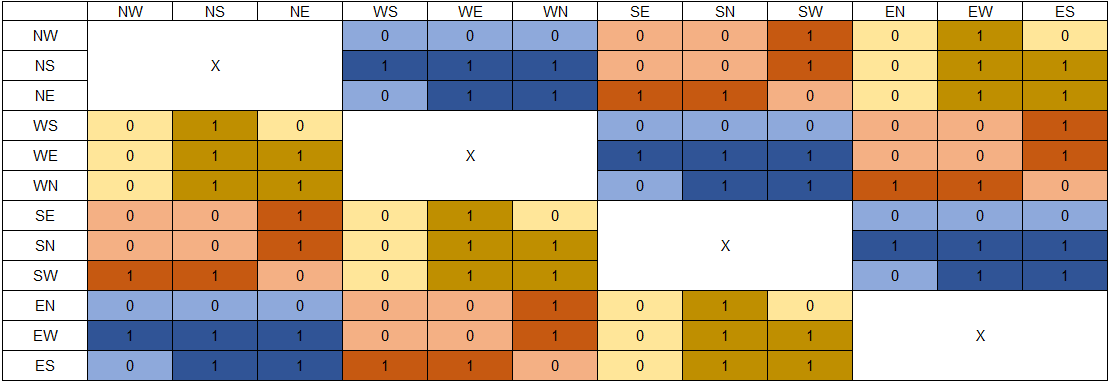
\includegraphics[scale=0.32]{collision table.png}}
    \caption{collision table with relative outputs}
    \label{table}
\end{figure}

Taking this specific concept of collision we noticed that we can simplify the output answers greatly, theoretically we could simplify the answers in three separate output blocks, but in order to have a much more simpler solution to VHDL, we just imagined the whole graph to be mirrored diagonally.

\subsubsection{Code Implementation}

When considering the required IO for our system, since the directions of each car will be represented by 4 bit system - we implemented 8 inputs in total, 4 bit directional representations for the two cars, which collision has to be checked. In terms of an output, we considered the most optimal solution is to have a single output, which would represent weather the collision is present or not.

Later on, we define all of the cardinal directions as signals, dedicating the 4 bit combination of each car to the direction representation. Hence, the original 4 bit input is just to represent the 12 possible directions, from which a car could come from and go to. Since we define that for 2 separate cars, each of them have a unique representation and so overall we have 24 directional signals defined.

Finally, we represent the logic of the collision table to the VHDL by expressing solutions, when the main output is considered to be equals to one. For instance, taking a look at the Figure \ref{table} we see, that if the first car comes from west to south and the second car is coming from north to south, then our collision, in this term our output is one. This is done with a all of the cases, where the collision is considered to happen and as referred before, since the graph is repetitive, only half of the solutions have to be implemented. Hence having this defined concludes the code implementation of VHDL

\subsubsection{ModelSIM results}



\subsection{FreeRTOS Implementation}



\section{Simulation Results}


\begin{thebibliography}{00}
\bibitem{b1} G. Eason, B. Noble, and I. N. Sneddon, ``On certain integrals of Lipschitz-Hankel type involving products of Bessel functions,'' Phil. Trans. Roy. Soc. London, vol. A247, pp. 529--551, April 1955.
\bibitem{b2} J. Clerk Maxwell, A Treatise on Electricity and Magnetism, 3rd ed., vol. 2. Oxford: Clarendon, 1892, pp.68--73.
\bibitem{b3} I. S. Jacobs and C. P. Bean, ``Fine particles, thin films and exchange anisotropy,'' in Magnetism, vol. III, G. T. Rado and H. Suhl, Eds. New York: Academic, 1963, pp. 271--350.
\bibitem{b4} K. Elissa, ``Title of paper if known,'' unpublished.
\bibitem{b5} R. Nicole, ``Title of paper with only first word capitalized,'' J. Name Stand. Abbrev., in press.
\bibitem{b6} Y. Yorozu, M. Hirano, K. Oka, and Y. Tagawa, ``Electron spectroscopy studies on magneto-optical media and plastic substrate interface,'' IEEE Transl. J. Magn. Japan, vol. 2, pp. 740--741, August 1987 [Digests 9th Annual Conf. Magnetics Japan, p. 301, 1982].
\bibitem{b7} M. Young, The Technical Writer's Handbook. Mill Valley, CA: University Science, 1989.
\end{thebibliography}

\end{document}
